\documentclass[11pt]{standalone}
\usepackage{amssymb}
\usepackage{amsmath}
\usepackage[no-math]{fontspec}
\usepackage{unicode-math}
\usepackage{libertinus}
\usepackage{pgf,xcolor}
\usepackage{tikz}
\usetikzlibrary{arrows.meta, backgrounds}
\usepackage{pgfplots}
\pgfplotsset{compat=newest}

\definecolor{my_darkgray}{HTML}{484949}
\definecolor{my_lightgray}{HTML}{F3F4F4}
\definecolor{my_darkblue}{HTML}{005A94}
\definecolor{my_lightblue}{HTML}{CCDEE9}
\definecolor{my_yellow}{HTML}{FFEC7F}
\definecolor{my_red}{HTML}{E60000}
\definecolor{my_orange}{HTML}{E87846}

\begin{document}
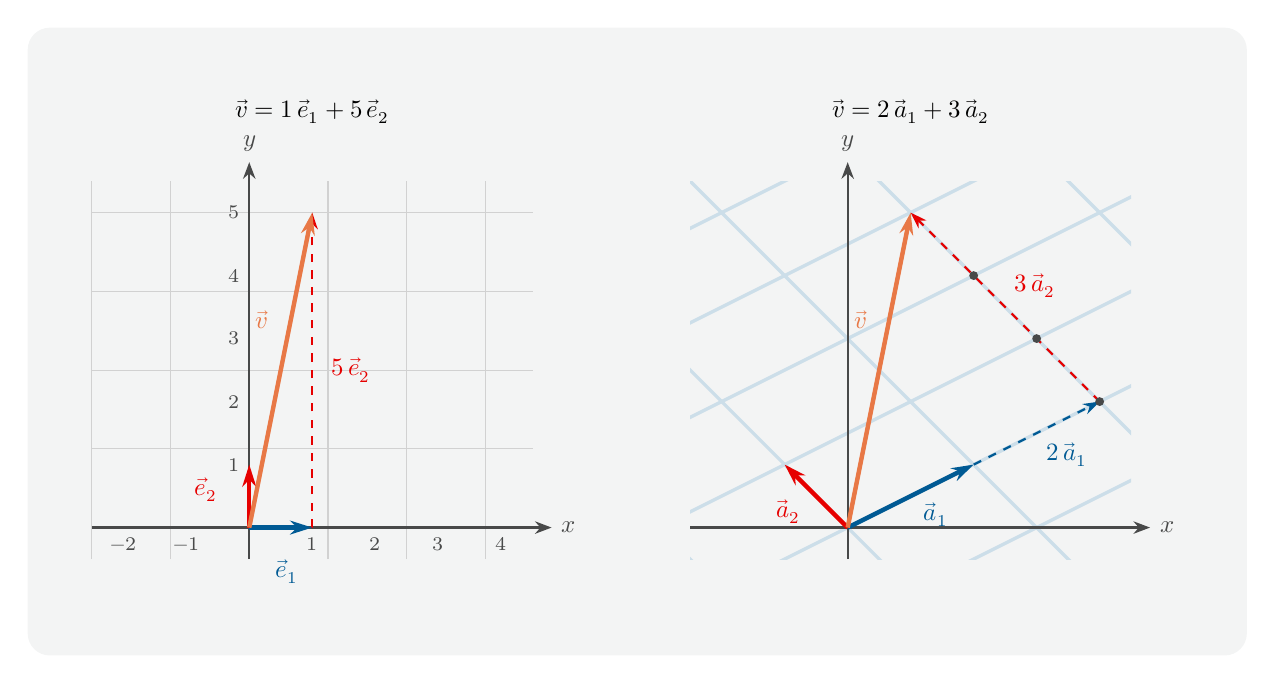
\begin{tikzpicture}[
    show background rectangle,
    background rectangle/.style={fill=my_lightgray, rounded corners=8pt},
    inner frame sep=0.8cm,
    x=0.8cm, y=0.8cm,
    vec/.style={-{Stealth[length=8pt, width=5pt]}, ultra thick},
    weg/.style={-{Stealth[length=6pt, width=4pt]}, thick, dashed}
]

% ---------------------------------------------------------------
%  Derselbe Vektor v = (1, 5) in zwei Basen:
%    links:  kanonische Basis,   v = 1 e1 + 5 e2
%    rechts: a1 = (2, 1), a2 = (-1, 1),   v = 2 a1 + 3 a2
% ---------------------------------------------------------------

% ===== Linkes Teilbild: kanonische Basis =====
\begin{scope}
    \draw[my_darkgray!25, thin] (-2.5, -0.5) grid (4.5, 5.5);
    \draw[-{Stealth[length=6pt]}, thick, my_darkgray] (-2.5, 0) -- (4.8, 0)
        node[right, font=\small] {$x$};
    \draw[-{Stealth[length=6pt]}, thick, my_darkgray] (0, -0.5) -- (0, 5.8)
        node[above, font=\small] {$y$};
    \foreach \x in {-2, -1, 1, 2, 3, 4}
        \node[below, font=\scriptsize, my_darkgray] at (\x, 0) {$\x$};
    \foreach \y in {1, ..., 5}
        \node[left, font=\scriptsize, my_darkgray] at (0, \y) {$\y$};

    % Weg 1 e1 + 5 e2
    \draw[weg, my_red] (1, 0) -- (1, 5);
    \node[right, font=\small, my_red] at (1.15, 2.5) {$5\,\vec{e}_2$};

    % Basisvektoren
    \draw[vec, my_darkblue] (0, 0) -- (1, 0);
    \draw[vec, my_red] (0, 0) -- (0, 1);
    \node[below, font=\small, my_darkblue] at (0.6, -0.35) {$\vec{e}_1$};
    \node[left, font=\small, my_red] at (-0.35, 0.6) {$\vec{e}_2$};

    % Vektor v
    \draw[vec, my_orange] (0, 0) -- (1, 5);
    \node[left, font=\small, my_orange] at (0.45, 3.3) {$\vec{v}$};

    \node[font=\small] at (1, 6.6)
        {$\vec{v} = 1\,\vec{e}_1 + 5\,\vec{e}_2$};
\end{scope}

% ===== Rechtes Teilbild: Basis a1, a2 =====
\begin{scope}[xshift=7.6cm]
    % Gitter der neuen Basis: Geraden lambda_1 = k und lambda_2 = k
    \begin{scope}
        \clip (-2.5, -0.5) rectangle (4.5, 5.5);
        \foreach \k in {-3, ..., 6} {
            \draw[my_lightblue, very thick]
                ({2*\k + 4}, {\k - 4}) -- ({2*\k - 8}, {\k + 8});
            \draw[my_lightblue, very thick]
                ({-\k - 8}, {\k - 4}) -- ({-\k + 12}, {\k + 6});
        }
    \end{scope}
    \draw[-{Stealth[length=6pt]}, thick, my_darkgray] (-2.5, 0) -- (4.8, 0)
        node[right, font=\small] {$x$};
    \draw[-{Stealth[length=6pt]}, thick, my_darkgray] (0, -0.5) -- (0, 5.8)
        node[above, font=\small] {$y$};

    % Weg 2 a1 + 3 a2
    \draw[weg, my_darkblue] (2, 1) -- (4, 2);
    \draw[weg, my_red] (4, 2) -- (1, 5);
    \node[below right, font=\small, my_darkblue] at (3, 1.5) {$2\,\vec{a}_1$};
    \node[above right, font=\small, my_red] at (2.5, 3.5) {$3\,\vec{a}_2$};
    \foreach \p in {(4, 2), (3, 3), (2, 4)}
        \fill[my_darkgray] \p circle (1.6pt);

    % Basisvektoren
    \draw[vec, my_darkblue] (0, 0) -- (2, 1);
    \draw[vec, my_red] (0, 0) -- (-1, 1);
    \node[below, font=\small, my_darkblue] at (1.4, 0.55) {$\vec{a}_1$};
    \node[below left, font=\small, my_red] at (-0.6, 0.6) {$\vec{a}_2$};

    % Vektor v
    \draw[vec, my_orange] (0, 0) -- (1, 5);
    \node[left, font=\small, my_orange] at (0.45, 3.3) {$\vec{v}$};

    \node[font=\small] at (1, 6.6)
        {$\vec{v} = 2\,\vec{a}_1 + 3\,\vec{a}_2$};
\end{scope}

\end{tikzpicture}
\end{document}
